\chapter{Application}
\label{application}
%#############################################################################################

In this chapter, we are trying to apply the algorithms that are described and implemented in~\ref{implementation} to various datasets: \textit{usps}, \textit{banana}, \textit{fishbowl}, \textit{swissroll} and \textit{flatroll}.

\section{Assignment 4: PCA}
\label{assignment4}

This assignment asks us to apply \textit{PCA} to the \textit{usps} data set and visualizing the results. The \textit{usps} data set consists of 2007 images with the dimension of \textit{16 x 16}. The images are hand-written digits of zero to nine, which can be viewed as classes. Firstly, i separate the data set according to each digit into ten classes and then applied \textit{PCA} to each class. The \textit{PCA} was applied to the original data set and noisy data set.

\subsection{Original Data Set}
\label{ass4:original}

PCA was applied to each class and then the results were visualized. As depicted in Figure~\ref{fig:pcaOriginal05} and \ref{fig:pcaOriginal69}, the following were visualized:

\begin{itemize}
	\item All principle values (as bar plot).
	\item The largest 25 principal values (as bar plot).
	\item The first 5 principal directions (as images).
\end{itemize}

From the visualization, it can be obtained that the information of the data set is only represented by a small subset of principal components, about five to ten components. 

\begin{figure}[h!]
	\centering
	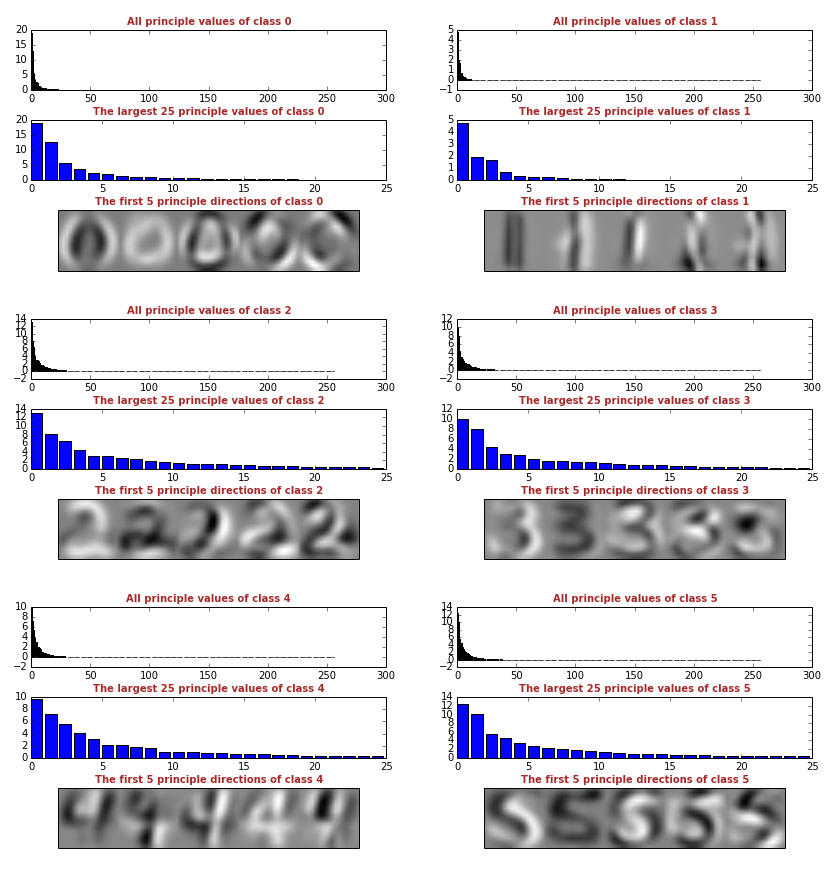
\includegraphics[scale=0.4983]{normalpca_0-5}
	\caption{Principal components of usps original data set for class 0 - 5}
	\label{fig:pcaOriginal05}
\end{figure}

\begin{figure}[h!]
	\centering
	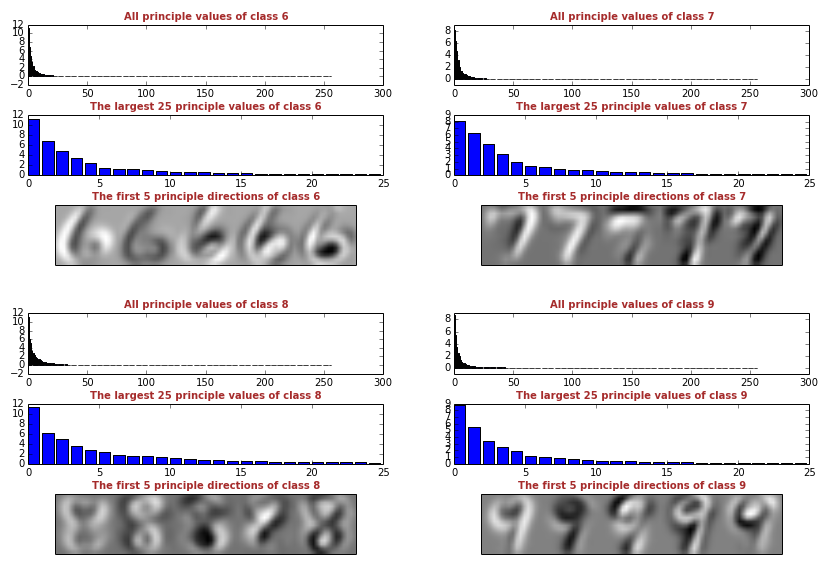
\includegraphics[scale=0.4983]{normalpca_6-9}
	\caption{Principal components of usps original data set for class 6 - 9}
	\label{fig:pcaOriginal69}
\end{figure}

\subsection{Noisy Data Set}
\label{ass4:noisy}

To make it more challenging, some noised are added to the original data set. There are three noise scenarios: \textit{low gaussian noise}, \textit{high gaussian noise} and \textit{outliers}.

For the \textit{low gaussian noise}, standard deviation used to generate the noise is 0.25, whereas for \textit{high gaussian noise} and \textit{outliers}, standard deviations of 0.55 and 1.25 are used, respectively. The same steps as in Subsection~\ref{ass4:original} are performed for all noisy data sets. The visualization is depicted in Figure~\ref{fig:pcaModerate05} to \ref{fig:pcaExtreme69}.

\begin{figure}[h!]
	\centering
	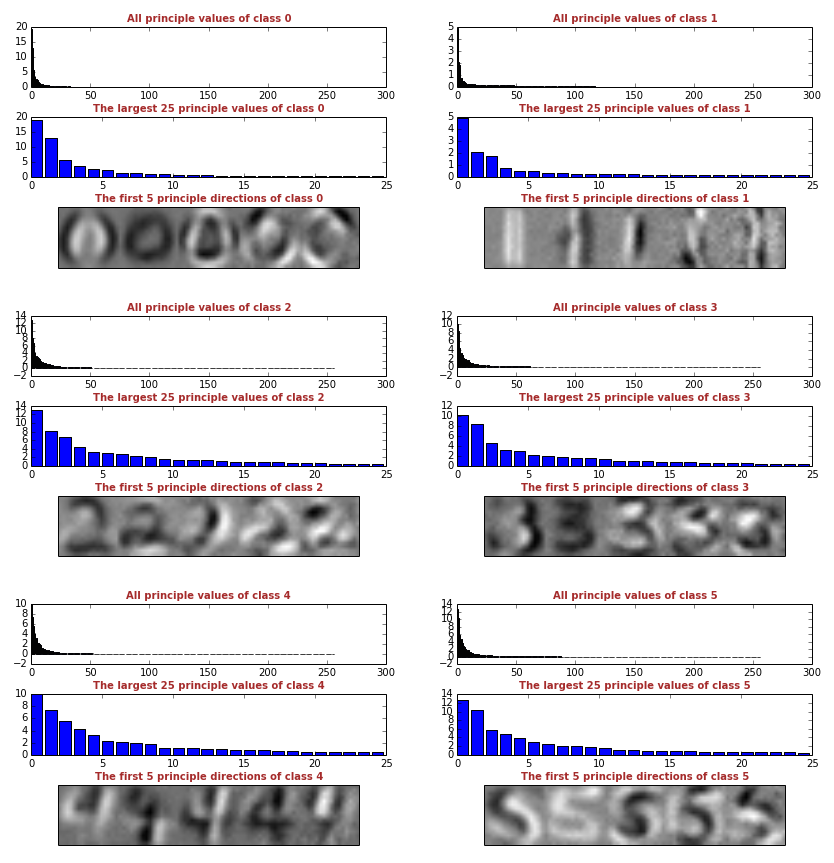
\includegraphics[scale=0.4983]{moderately_noisy_0-5}
	\caption{Principal components of moderately noisy data set for class 0 - 5}
	\label{fig:pcaModerate05}
\end{figure}

\begin{figure}[h!]
	\centering
	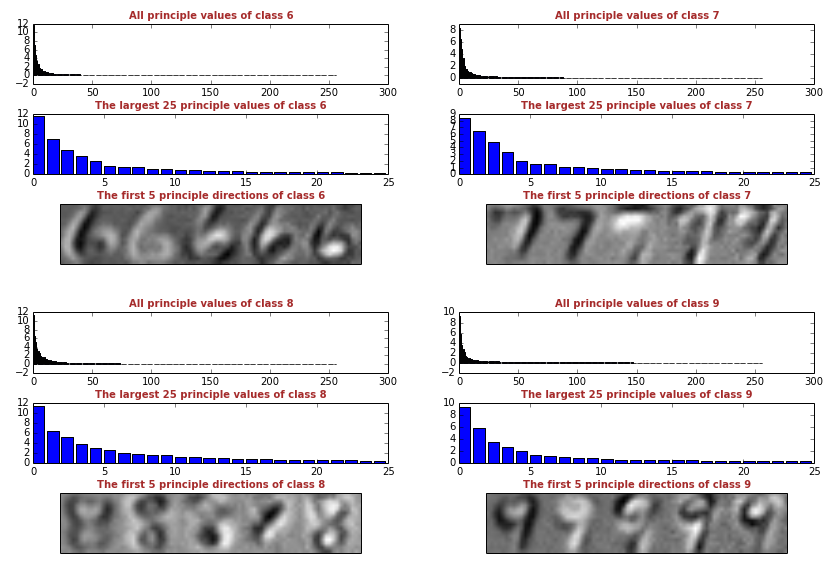
\includegraphics[scale=0.4983]{moderately_noisy_6-9}
	\caption{Principal components of moderately noisy data set for class 6 - 9}
	\label{fig:pcaModerate69}
\end{figure}

\begin{figure}[h!]
	\centering
	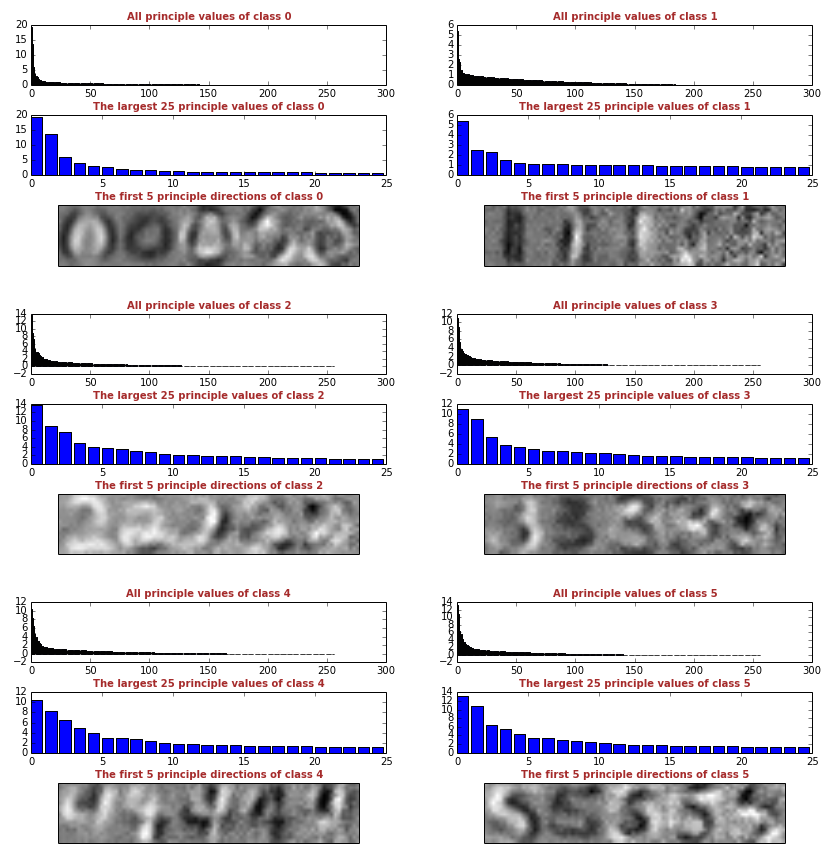
\includegraphics[scale=0.4983]{very_noisy_0-5}
	\caption{Principal components of very noisy data set for class 0 - 5}
	\label{fig:pcaVery05}
\end{figure}

\begin{figure}[h!]
	\centering
	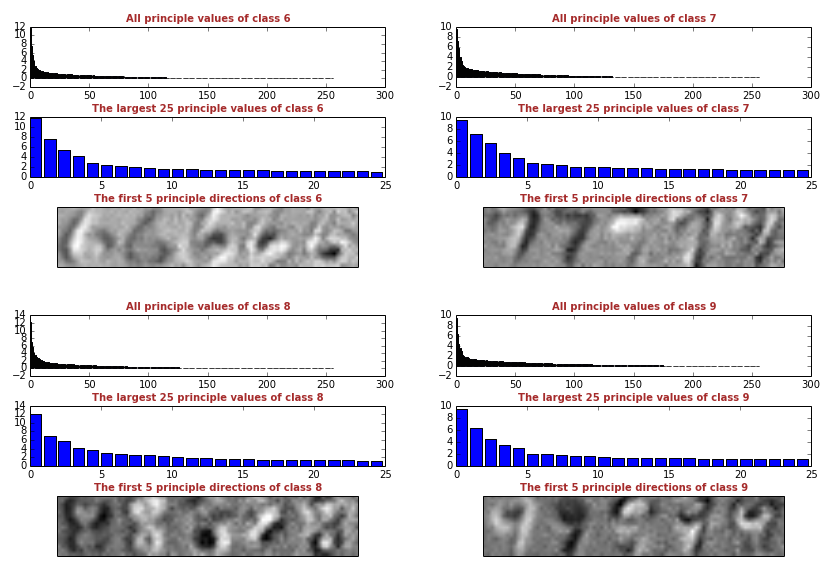
\includegraphics[scale=0.4983]{very_noisy_6-9}
	\caption{Principal components of very noisy data set for class 6 - 9}
	\label{fig:pcaVery69}
\end{figure}

\begin{figure}[h!]
	\centering
	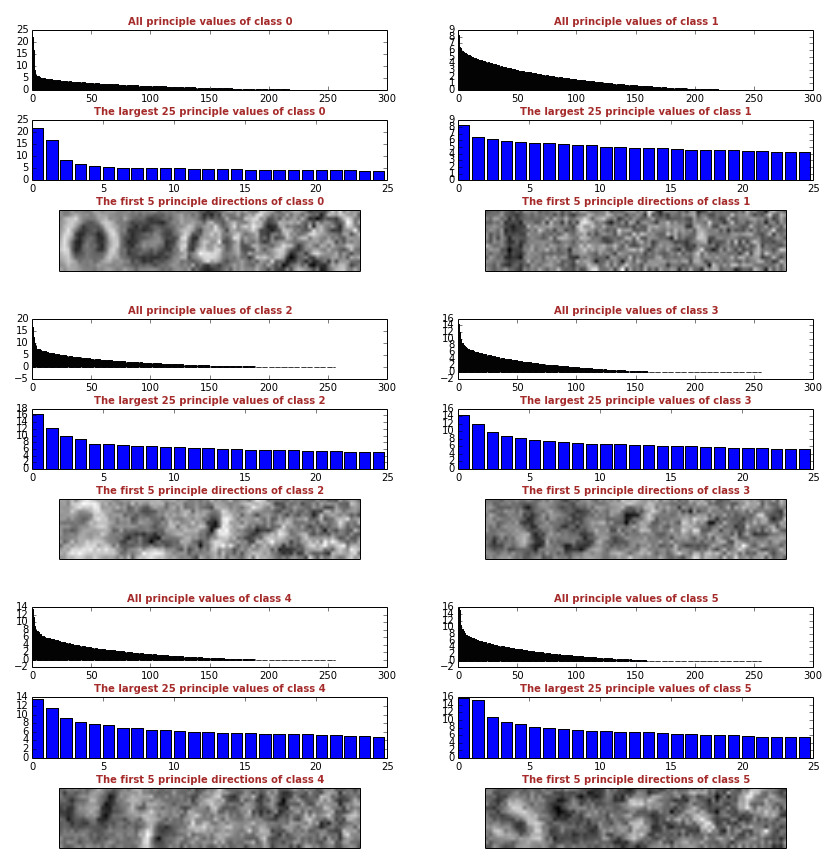
\includegraphics[scale=0.4983]{extremely_noisy_0-5}
	\caption{Principal components of extremely noisy data set for class 0 - 5}
	\label{fig:pcaExtreme05}
\end{figure}

\begin{figure}[h!]
	\centering
	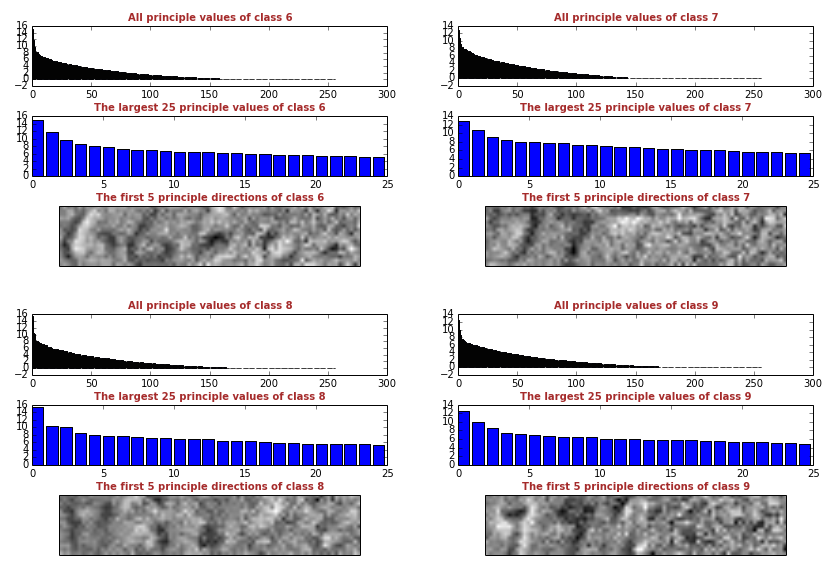
\includegraphics[scale=0.4983]{extremely_noisy_6-9}
	\caption{Principal components of extremely noisy data set for class 6 - 9}
	\label{fig:pcaExtreme69}
\end{figure}

It can be obtained that the information of the data set is now represented by a bigger number of principal components. The noisier a data set is, the bigger the number of principal components is needed to represent the information of the data set.

Figure~\ref{fig:pcaExamples} shows ten images of the original data, noisy data, and their reconstruction (denoised) data using \textit{PCA}. The number of components \textit{m} used for \textit{moderately} noisy images is 11, for \textit{very} noisy images is 75 and for \textit{extremely} noisy images is 150.

\begin{figure}[h!]
	\centering
	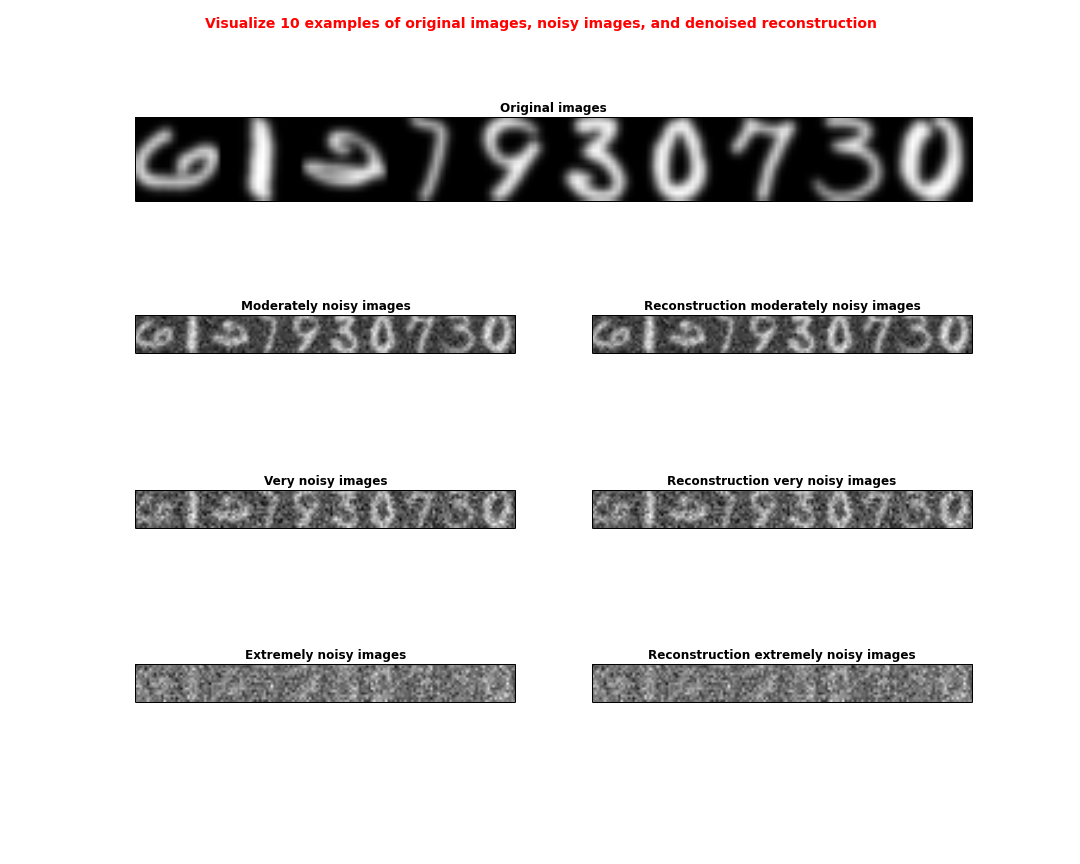
\includegraphics[scale=0.4983]{pcaexamples}
	\caption{Examples of some original, noisy and reconstruction images}
	\label{fig:pcaExamples}
\end{figure}

%#############################################################################################
\section{Assignment 5: Outlier Detection Using $\gamma$-Index}
\label{assignment5}

In this assignment, the $\gamma$-index method is used to detect outliers. The data set used is \textit{banana} data set. The positive class of the data set is used as \textit{inliers}, to which the negative class is added as outliers. The $\gamma$-index method is used to detect outliers with contamination rates of 1%, 5%, 10% and 25% relative to the positive class.

%#############################################################################################

\section{Assignment 6: LLE}
\label{assignment6}

%#############################################################################################

\section{Assignment 7: LLE With Noise}
\label{assignment7}